\documentclass[]{article}

\usepackage{amsmath}
\usepackage{mathrsfs}
\DeclareMathAlphabet{\mathpzc}{OT1}{pzc}{m}{it}

\usepackage{graphicx}
\usepackage{subfig}
\usepackage{wrapfig}
\usepackage{enumitem}


\DeclareMathOperator{\di}{d\!}
\newcommand*\Eval[3]{\left.#1\right\rvert_{#2}^{#3}}

%opening
\title{Nonlinear Decoherence of an Offset Waterbag}
\author{Christopher Hall}

\begin{document}

\maketitle

\begin{abstract}

\end{abstract}

\section{Introduction}
% TODO: No coupling in this formulation

The goal of this work is to provide a model for the centroid motion of bunch undergoing 
nonlinear decoherence. To begin we assume that the bunch starts out with some 
displacement $\Delta x$ along one transverse axis at turn $N=0$. We will then find a 
representation of  $\hat{x}(N)$ the normalized centroid position $\left\langle x 
\right\rangle 
/ \sigma_x$ as a function of turn number. 

We begin by following SSC-N-360 and describe particle motion in the coordinates $ a = 
\sqrt{\beta_x \varepsilon_x} / \sigma_x$ and $\varphi$, for the amplitude and initial phase 
of a 
particle. This means that the actual particle displacement is then $x = \sigma_x a cos(2 \pi 
\nu N + \varphi)$. 

Because of the presence of the nonlinear element there will be amplitude-dependence in 
the particle tune. may be characterized in terms of
a unitless strength parameter $t$ and geometric scale factor $c$, with units of
$m^\frac{1}{2}$, that describes the location of two singularities in the x-plane. The first
few terms of the multipole expansion for the elliptic potential in normalized coordinates
$\hat{x}, \hat{y} = x / \sqrt{\beta}, y / \sqrt{\beta}$ are given by %\cite{valishev:napac16}
\begin{equation} \label{eq:expansion}
U(\hat{x}, \hat{y}) = \frac{-t}{c^2} \, Im\left\lbrace (\hat{x}+i\hat{y})^2 +
\frac{2}{3c^2}(\hat{x} + i\hat{y})^4 + \right.
\left. \frac{8}{15c^4}(\hat{x}+i\hat{y})^6 + ... \right\rbrace.
\end{equation}
Note: this expansion is only valid in the region $\sqrt{\hat{x}^2 +\hat{y}^2} < c$. Because 
of the form of the potential we expect to see just the even 
terms in amplitude effecting the tune.

\section{Nonlinear Decoherence and the Centroid}

Due to the octupole and higher terms in the potential the tune $\nu$ will have an 
amplitude dependence of the form

\begin{equation} \label{eq:tune}
\nu = \nu_0 - \sum_{i=1} \mu_i a^{2i},
\end{equation}

where $\nu_0$ is the unperturbed tune and $\mu_i$ are coefficients determined by the 
octupole, duodecapole, etc. multipole components in the nonlinear element. The 
calculation of these coefficients becomes cumbersome beyond the lowest order. This is a 
major obstacle to the use of the formulation developed here. This issue will be discussed 
further on.

This amplitude-dependent tune will result in particles having a phase shift each turn of
\begin{equation}
	\Delta \varphi(a, N) = -2 \pi N \sum_{i=1} \mu_i a^{2i},
\end{equation}
when compared to the unperturbed phase advance $\nu_0$. From this the centroid 
motion for a distribution $\rho(a, \varphi)$ as a function of turn number in a lattice with 
some nonlinearities will be

\begin{equation} \label{eq:centroid}
\hat{x}(N) = \int_{0}^{\infty}da \int_{0}^{2\pi}d\varphi \, a cos(\varphi) \rho(a,
\varphi -
2\pi N \nu).
\end{equation}

\section{Calculation for a Waterbag Distribution}

Because all our simulation data we will compare to uses a waterbag distribution we are 
first interested in the calculation of Eq. \ref{eq:centroid} for such a distribution. here we 
define a 'waterbag' according to the definition of Reiser, that is the bunch has a uniform 
distribution of particle amplitudes from 0 to some cutoff, that is

\begin{equation} \label{eq:waterbag}
\rho(a, \varphi) =
\left\{
\begin{array}{lr}
1 &  a \leq 1 \\
0 &  a > 1
\end{array}
\right.
\end{equation}. 

We then assume that the distribution starts out with a centroid offset, in our normalized 
coordinates is, $Z = \Delta x / \sigma_x$. This offset waterbag then takes form

\begin{equation} \label{eq:offset_wb}
\rho(a, \varphi) =
\left\{
\begin{array}{lr}
\frac{1 + Z^2 - 2Zcos(\varphi)}{\pi} &  0 < a \leq 1 \\
0 &  a > 1 \, \,o \, \,r a < 0
\end{array}
\right.
\end{equation}

Inserting Eq. \ref{eq:offset_wb} in Eq. \ref{eq:centroid} we can make a convenient change 
of variable $u=a^2$ and perform the integration in $\varphi$, resulting in
%NOTE: My notes do not agree on the sign of these two terms so I am following the code 
%in decoherence.py, since it's been validated against simulations

\begin{equation}
	\hat{x}(N) = \pi Z \int_{0}^{1} du \,\, cos(2 \pi \nu_0 N)cos(\Delta \varphi(u, N)) + sin(2 
	\pi 
	\nu_0 N) sin(\Delta \varphi(u, N))
\end{equation}

A second change of variable $\hat{u} = 2 \pi N u$ is then made to assist in numerical 
integration down the road. The general result for the centroid motion is then

\begin{equation} \label{eq:general_centroid}
\hat{x}(N) = \frac{Z}{2 N} \int_{0}^{2\pi N} d\hat{u} \,\, cos(2 \pi \nu_0 N)cos(\Delta 
\varphi(u, 
N)) - 
sin(2 \varphi 
\nu_0 N) sin(\Delta \varphi(u, N))
\end{equation}

As a reminder the phase slip $\Delta \varphi$ has now become

\begin{equation} \label{eq:phase_slip_2} 
	\Delta \varphi(\hat{u}, N) = \sum_{i=1} \frac{\mu_i \hat{u}^{i}}{(2 \pi N)^{i - 1}}.
\end{equation}

We now have a general solution for our original problem, the centroid motion as a 
function of turn number. Quite nicely, this solution is not iterative, any turn can be 
calculated independently. This does aid speeding up the turn-by-turn centroid motion, 
however, this is where the good news stops. We still have a set of unknown coefficients 
$\mu_i$ that will depend on particulars of the nonlinear element in the lattice and must be 
iteratively derived from a perturbation method or found from numerical fitting. For this 
second option we can use simulation data from IOTA and fit up to the desired order (as 
well as $\nu_0$ possibly). However, this numerical method is greatly complicated by the 
highly-oscillatory nature of the integrand of Eq. \ref{eq:general_centroid}. As an example 
the integrand is plotted in Fig. \ref{fig:integrand} for two different values of $N$. For the 
case of $N=200$ the high-frequency oscillations tend to make the numerical integration 
both extremely slow and greatly limits accuracy in many cases.

\begin{figure}
	\centering
	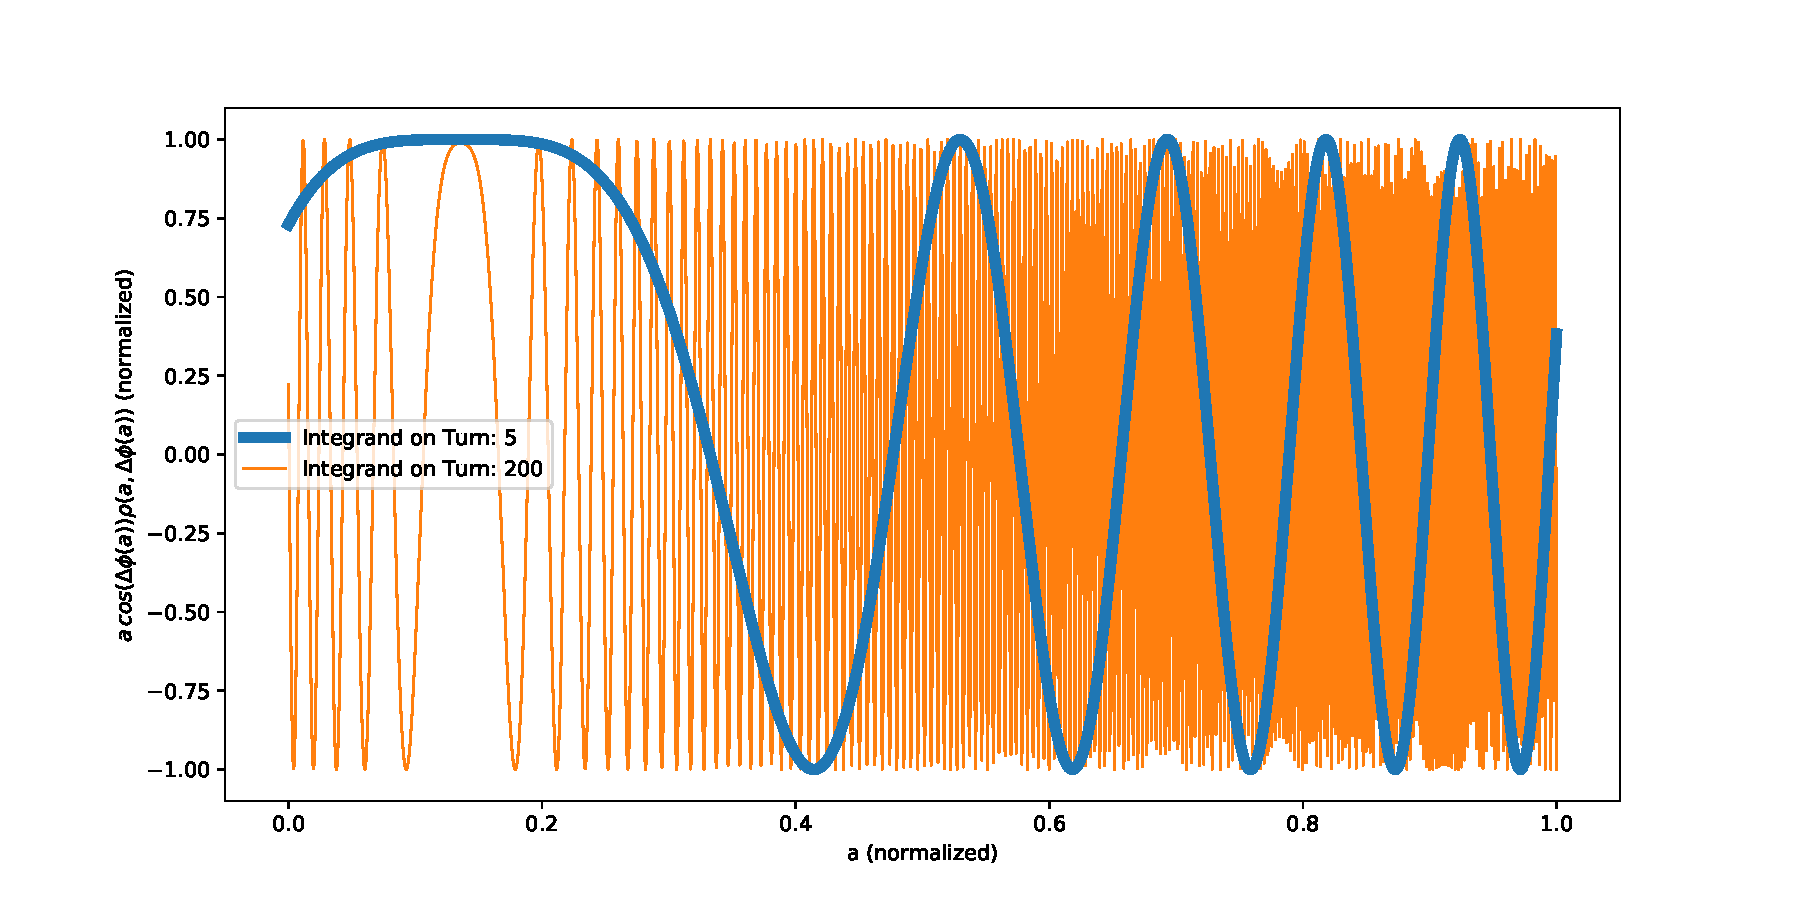
\includegraphics[width=\columnwidth]{co_figures/integrand_oscillation.pdf}
	\caption{Integrand of Eq. \ref{eq:general_centroid} on turn 5 and turn 100.}
	\label{fig:integrand}
\end{figure}

Evaluation of the general waterbag case, Eq. \ref{eq:general_centroid}, is available through 
the \texttt{rsbeams.rsphysics.decoherence} module. The general integration is performed 
with \texttt{scipy.integrate.quad} which in turns uses the Fortran QUADPACK library. 
(Note: This uses the Clenshaw-Curtis Quadrature, which has the possibility of introducing 
a weight function to the integrand that can ease integration of high-oscillatory functions. 
This has not been explored though.). For evaluating N turns we take advantage of the 
independent nature of each turn and use the \texttt{Pool} function from the 
\texttt{pathos.multiprocessing} package to parallelize the calculations. The standard 
\texttt{multiprocessing} library will not work in this instance as it is not able to be run 
from within a class instance and evaluate a method belonging to the class. The Pathos 
implementation does not have this limitation.

\subsection{Special Cases}

While the general evaluation of Eq. \ref{eq:general_centroid} does not appear analytically 
tractable there are two special cases. If we truncate $\Delta \varphi$ at $\hat{a}$ there is 
an exact analytic solution, in the case of truncating at $\hat{a}^2$ a solution can be found 
in terms of Fresnel integrals, which are relatively easy to calculate.

For just $i=1$ the exact solution is

\begin{equation}
	\hat{x}(N) = \frac{Z}{2 \pi N}\frac{cos(2 \pi \nu_0 N) sin(2 \pi N \mu_1) + 2sin(2\pi \nu_0 
	N) 
	sin^2(\pi N \mu_1)}{\mu_1}.
\end{equation}

With both $i=1,2$ the solution becomes

\begin{multline}
\hat{x}(\hat{u}, N) = \frac{Z}{\sqrt{8 \pi N^2 \mu_2}} \left[
C\left( \frac{\pi N \mu_1 +\mu_2 \hat{u} }{\sqrt{\pi^2 N \mu_2}} \right)
cos \left( \frac{\pi N \mu_1^2}{2 \mu_2} + 2 \pi N \nu_1 \right) \right. + \\
\left. \left. S\left( \frac{\pi N \mu_1 +\mu_2 \hat{u} }{\sqrt{\pi^2 N \mu_2}} \right)
sin \left( \frac{\pi N \mu_1^2}{2 \mu_2} + 2 \pi N \nu_1 \right)
\right] \right|_{0}^{2 \pi N},
\end{multline}
where $C$ and $S$ are the Fresnel integrals. The \texttt{rsbeams.rsphysics.decoherence} 
package includes both these representations and will automatically use them when 
appropriate.




\end{document}
